% =============================================================================
\section{Walkers and groups in the data}\label{sec:data}

\begin{figure*}[t]
\centering
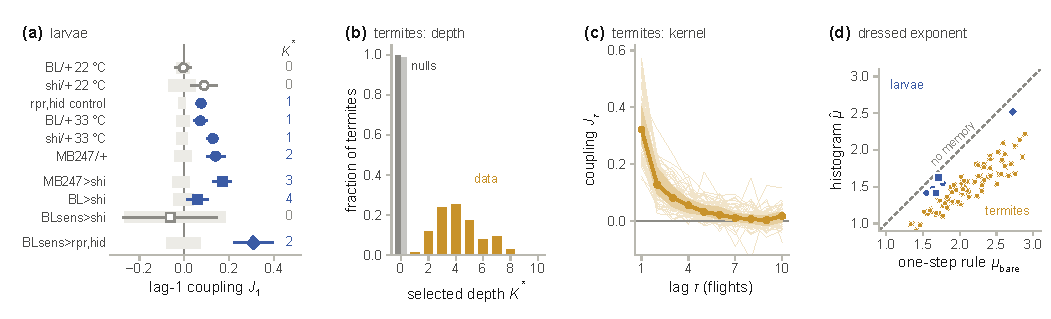
\includegraphics[width=\textwidth]{figs/fig3_walkers.pdf}
\caption{Single walkers. (a)~\emph{Drosophila} larvae: lag-1 coupling with one field per larva ($\pm2$ s.e.) and, on the right, the depth $K^*$ selected by BIC; filled symbols, $K^*>0$; grey bands, $\pm2$ s.d.\ over 30 within-larva permutations of the flights. Circles, controls; squares, neurons silenced with \emph{shibire}$^{ts}$; diamond, brain lobes and sensory neurons ablated (genotypes in Appendix~\ref{app:data}). (b)~Depth selected in each of 75 termites (ochre), and by the within-track permutation and pipeline nulls (grey), which select $K^*=0$. (c)~Memory kernel of the termites, from fits with $K=10$: single termites (thin lines), median and interquartile range. (d)~Exponent of the histogram of all flights, $\hat\mu$, against the exponent of the one-step rule, $\mub$, for the larval conditions with memory (medians over larvae, symbols as in (a)) and for each termite; dashed, the diagonal of renewal walkers.}
\label{fig:walkers}
\end{figure*}

All single walkers go through the same pipeline (Appendix~\ref{app:data}): flights are cut out of each track with a corridor of half-width $\varepsilon=0.5$\,mm, nearly collinear pieces are merged, $\lmin=1$\,mm, and $\lmax$ is the longest flight of the condition (larvae) or of the track (termites).

\subsection{\emph{Drosophila} larvae}\label{sec:larvae}

Sims \emph{et al.}~\cite{Sims2019} filmed \emph{Drosophila} larvae crawling for up to one hour on plain agar, without odor, light or food, and found L\'evy-like flight statistics that persisted when large parts of the nervous system were switched off. Neurons were targeted with the GAL4--UAS system. The driver BL expresses in the brain lobes and in part of the subesophageal ganglion, BLsens in the same regions and in all sensory neurons, MB247 in the mushroom bodies, a center of learning and memory. The targeted neurons were either silenced with \emph{shibire}$^{ts}$, a temperature-sensitive mutant of dynamin that blocks synaptic transmission above about 30\,$^\circ$C~\cite{Kitamoto2001} (the larvae were tested at 33\,$^\circ$C, some controls also at the permissive 22\,$^\circ$C), or killed by expressing the pro-apoptotic genes \emph{reaper} and \emph{hid} (\emph{rpr,hid}). Larvae that carry only the driver (BL/+, MB247/+) or only the effector (shi/+) are controls. Because the L\'evy statistics survived without brain and senses, Sims \emph{et al.} traced them to the central pattern generator for locomotion in the ventral nerve cord. In an environment controlled so tightly, these data are ideal to ask whether the intrinsic walk of the larva is a renewal process. The 241 tracks with at least 17 flights, 20\,948 flights in ten conditions, are fitted condition by condition with one field per larva and $K\le6$ (Table~\ref{tab:larvae}).

Renewal is rejected in seven of the ten conditions [\figref{fig:walkers}(a)]. The memory is positive, long flights tending to follow long flights, and short, one to four flights deep. It does not depend on how the flights are cut, and in six of the seven conditions it survives when the field of each larva is re-estimated every 25 flights, so it is not a slow drift of the exponent; in BL$>$shi it disappears, and is better described as a slow modulation (Appendix~\ref{app:data}). The nulls are clean: within-larva permutations select $K^*>0$ in 1 of 300 surrogates, and the pipeline null in none of 50. Of the three conditions compatible with renewal, BLsens$>$shi has too few flights (349) to decide, and shi/+ at 22\,$^\circ$C has a lag-1 coupling three standard errors from zero that BIC does not retain; only BL/+ at 22\,$^\circ$C shows no trace of memory.

The memory is strongest in the BLsens$>$\emph{rpr,hid} larvae, whose brain lobes and sensory neurons are dead: $J_1=0.31\pm0.05$, eight standard deviations from the permutation null. In the logic of Ref.~\cite{Sims2019}, the memory between flights is generated below the brain, together with the L\'evy-like statistics, and needs neither the brain nor sensory feedback.

Six of the seven conditions with memory sit at $\Phi\simeq0.7$--1.0 [\figref{fig:overview}(c)], close to the spinodal and about half way to condensation; BL$>$shi, whose memory is a slow modulation, sits at 0.35. Replacing the longest observed flight by the side or the diagonal of the $240\times240$\,mm arena changes $\Phi$ by at most 0.2, because $\mub$ and $J_1$ readjust with $L$. The exponent is visibly dressed [\figref{fig:walkers}(d)]: the one-step rule has $\mub=1.54$--1.77 (2.72 for the ablated larvae), the histogram $\hat\mu=1.41$--1.63 (2.52), and the stationary law of the fitted chains reproduces every observed $\hat\mu$ within 0.03. Over the full range of flights a truncated log-normal law describes the histogram better than a truncated power law in eight conditions out of ten, so ``L\'evy'' here means at most two decades of approximate scaling; the memory is the same with either single-flight law (Appendix~\ref{app:data}).

\subsection{Termites}\label{sec:termites}

Castiblanco \emph{et al.}~\cite{Castiblanco2019} tracked focal workers of the termite \emph{Cornitermes cumulans} for 6\,h at 2\,Hz, in Petri dishes about 49\,mm across, together with nestmates at different densities. Each of the 75 tracks contains 673 to 12\,091 flights (median 3746), enough to analyze every termite on its own, with $K\le10$.

Every termite remembers. BIC selects a depth between 1 and 8, with a median of 4 [\figref{fig:walkers}(b)], and the lag-1 coupling is positive in all 75 tracks, $J_1=0.34\pm0.10$ (mean $\pm$ s.d.\ over termites); the memory kernel decays over about five flights [\figref{fig:walkers}(c)]. Within-track permutations select memory in 0.3\% of the surrogates, and the pipeline null gives $K^*=0$ in 74 of 75 tracks. With fields re-estimated every 50 or 25 flights the lag-1 coupling stays significant in every termite (median $z=21$ and 18, minimum 6.3).

Termites, like many insects, keep close to walls, a behavior known as thigmotaxis: they spend 30\%, 59\% and 79\% of the time within 3, 6 and 9\,mm of the wall of the dish. The memory could therefore have been geometric, long flights along the wall following each other. It is not. Adding the wall state of each flight as a covariate leaves the lag-1 coupling unchanged (median 0.42 without and 0.41--0.43 with it, for the three bands) and the selected depth unchanged (median 4), and on runs of consecutive flights far from the wall the coupling is even larger, $J_1\simeq0.49$ (Appendix~\ref{app:data}).

The termites sit further into the phase diagram than the larvae, at $\Phi=1.0$--3.5 (median 1.46) [\figref{fig:overview}(c)]: all of them beyond the spinodal, and 7\% beyond the condensation line, consistent with an arena that bounds their longest flights. Their exponents are the most dressed [\figref{fig:walkers}(d)]. The one-step rule has a median $\mub=2.07$, the histogram $\hat\mu=1.49$: read from the histogram, the exponent is off by more than half a unit. The apparent exponent grows with the density of nestmates (medians 1.18, 1.51 and 1.59 at densities 0.08, 0.12 and 0.20).

\begin{figure*}[t]
\centering
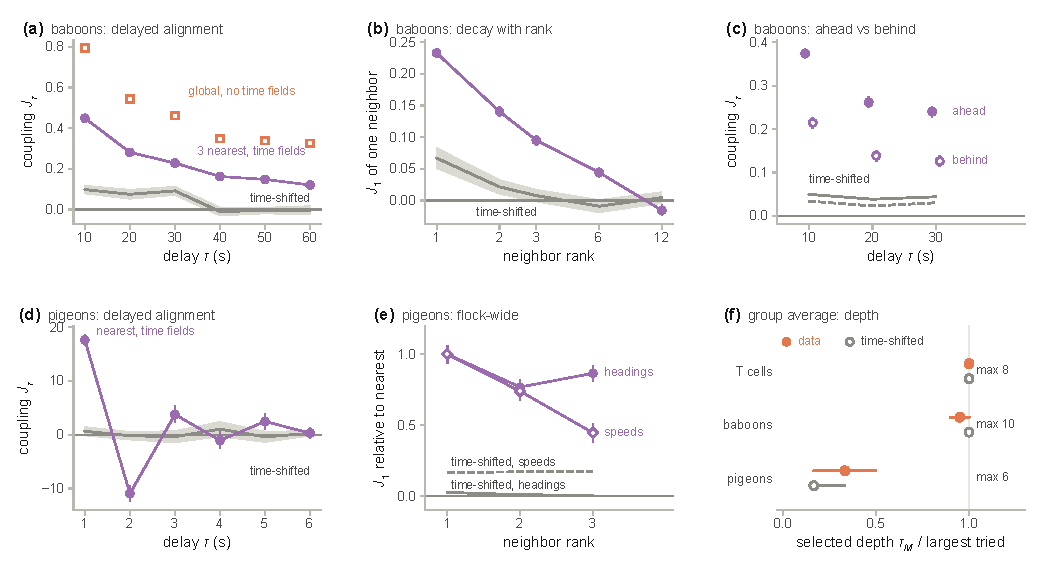
\includegraphics[width=\textwidth]{figs/fig4_groups.pdf}
\caption{Groups. Top: a wild baboon troop~\cite{StrandburgPeshkin2015} (14 days, clock 10\,s, headings). (a)~Couplings of a baboon's heading to the mean heading of its three nearest neighbors at delay $\tau$, with baboon and time fields ($\pm2$ s.e.); grey, mean $\pm2$ s.d.\ over 20 troops in which every baboon is shifted in time; open squares, a global coupling without time fields. (b)~Coupling at 10\,s to a single neighbor of given distance rank, all ranks fitted jointly. (c)~Couplings to the neighbors ahead (filled) and behind (open) along the group heading, among the six nearest; grey, time-shifted troops (solid, ahead; dashed, behind). Bottom: homing-pigeon flocks~\cite{MehlhausenFranks2025} (41 releases, clock 1\,s). (d)~As (a), for the nearest neighbor. (e)~Couplings at 1\,s to a single neighbor of given rank, relative to the nearest, for headings (filled) and log-speeds (open); grey, time-shifted flocks. (f)~Depth $\tau_M$ selected by the group-average analysis, as a fraction of the largest depth tried, on the data (coral) and on time-shifted units (grey): median and interquartile range over days (baboons), releases (pigeons) and surrogates; for the T cells, 16 fish pooled.}
\label{fig:groups}
\end{figure*}

\subsection{Baboons and pigeons}\label{sec:realgroups}

A wild troop of olive baboons~\cite{StrandburgPeshkin2015,Crofoot2015data}, 26 animals tracked by GPS every second for 14 days, is a group whose members share a clock and whose positions define neighbors. We use a clock of 10\,s, each day being a co-recorded group ($6\times10^4$ frames in all), and both variables, log-speeds and headings, a heading being defined for steps of at least 1\,m (Appendix~\ref{app:data}). Analyzed through its group average, the troop has a long memory: the selected depth has a median of 9.5 delays over days for headings and is 10, the largest tried, for log-speeds. Time-shifted baboons give the same depths, 10 in 82\% of the day replicates for headings and in all of them for log-speeds [\figref{fig:groups}(f)]. The depth is thus each baboon's own persistence ($\hat a_1=0.70$ for headings, 0.23 for log-speeds), seen through the average as in Eq.~\eqref{eq:aggregation}.

The self\,+\,social model, with baboon and time fields, finds in addition a delayed alignment with the three nearest neighbors, $J_1=0.449\pm0.007$ at 10\,s, which decays over a minute [\figref{fig:groups}(a)]; on a clock of 30\,s the first coupling is the same, $0.447\pm0.008$. Three controls single it out. Time-shifted baboons keep a coupling of $0.10\pm0.01$ at the shortest delays, because animals that pass the same place at different times head the same way, a field fixed in space that time fields cannot absorb; the data exceed it fourfold. The coupling lives at the nearest neighbors: $0.233\pm0.004$ with the single nearest, then 0.140, 0.095 and 0.044 with the second, third and sixth, and zero with the twelfth [\figref{fig:groups}(b)]. And it is asymmetric: neighbors ahead along the group heading weigh $0.374\pm0.006$, those behind $0.214\pm0.006$, against 0.050 and 0.034 for time-shifted baboons [\figref{fig:groups}(c)]. A baboon thus turns toward where its nearest neighbors, those ahead above all, were heading 10 to 30\,s earlier, in line with the following of initiators documented in this troop~\cite{StrandburgPeshkin2015}; a path walked first by those ahead would act in the same direction, and fields fixed in space would be needed to tell the two apart. Log-speeds tell the same story on a smaller scale, $J_1=0.052\pm0.002$ against $0.017\pm0.001$ for shifted baboons. Read with a global coupling and no time fields, the same headings give $J_1=0.79$ [\figref{fig:groups}(a), squares], the alignment plus the common motion of the troop.

Homing pigeons~\cite{MehlhausenFranks2025,MehlhausenFranks2025data}, three flocks released 41 times, form small groups of three to eight birds per frame, which we follow on a clock of 1\,s. On this scale flight is nearly ballistic, and a bird's heading is extrapolated from its last three, $\hat a_\tau=(185,-82,21)$, that is, from its direction and its rate of turn. The group-average analysis again returns the depths of time-shifted birds, 1 to 3\,s in 80\% of the releases against 91\% for shifted birds [\figref{fig:groups}(f)]. The self\,+\,social model couples each bird to its nearest neighbor with $J_\tau=(17.6\pm0.6,-11.0\pm0.8,3.8\pm0.8)$, against $(0.6\pm0.4,-0.2\pm0.4,-0.4\pm0.6)$ for shifted birds [\figref{fig:groups}(d)]. The alternating signs repeat those of own memory: a bird follows both the last heading of its neighbor and its last turn. In flocks this small the heading coupling does not decay over the three nearest neighbors, whereas speeds match the nearest one most [\figref{fig:groups}(e)]; log-speeds are coupled with $J_1=3.8\pm0.1$, against $0.5\pm0.2$ for shifted birds. Nor is the coupling stronger toward birds ahead ($3.5\pm0.3$ ahead, $5.3\pm0.3$ behind among the three nearest): pigeons follow their leaders with delays of fractions of a second~\cite{Nagy2010}, within one frame of this clock, and a model of delayed couplings sees only the interactions slower than its frame.

\subsection{A negative control: T cells}\label{sec:tcells}

T cells close the analysis as a negative control, first for single walkers. Jerison and Quake~\cite{Jerison2020} showed that the apparent heavy tails of their steps come from differences between cells, so any memory found with one field for all cells should be heterogeneity in disguise. It is. With one field for all cells, every group of T cells (and of \emph{Dictyostelium} amoebae from the same data set) shows deep memory, and it still does after the steps of each cell are shuffled ($K^*=5$--6 in 49 of 50 surrogates), which can only be heterogeneity. With one field per cell the shuffled data give $K^*=0$ in every surrogate, the memory of mouse T cells disappears, and zebrafish T cells and \emph{Dictyostelium} keep a short persistence ($J_1\simeq0.14$--0.15 per frame; Appendix~\ref{app:data}).

The same cells also test the group analysis. Zebrafish T cells co-recorded within each fish on a common clock of 45\,s (16 fish, 712 cells, 85\,016 steps) remember their own speed for about four frames ($\hat a_1\simeq0.20$). The group-average analysis selects a delay of 8 frames, the largest tried, and it selects the same delay in 20 of 20 time-shifted surrogates [\figref{fig:groups}(f)]: the delay is own memory. A weak coupling to the three nearest cells, $J_1=0.021\pm0.006$, vanishes once time fields are included, $0.005\pm0.007$; what remains is a drive shared within each fish. As far as the model can see, the cells do not interact.

The same model and the same controls thus return different answers for different groups: a delayed alignment of baboons with their nearest neighbors, stronger toward those ahead; a flock-wide coupling between pigeons, whose leader--follower delays are shorter than a frame; and no interaction between T cells. In none of the three could the answer be read off the group average, whose selected depth is in each case the own memory of the units.
